% グリッドを表示させるのは draft の時だけにすれば良い
%\documentclass[draft,a4j,11pt,papersize]{jsarticle}
% 印刷時には draft オプションを除けば良い。
\documentclass[a4j,11pt,papersize]{jsarticle}
% 
% graphicx パッケージには final を渡して、いつでも図が表示される
% ようにすると、labelfig の調整が容易になる。
\usepackage[final]{graphicx}
\usepackage{labelfig}
\begin{document}

\begin{figure}[htbp]
 \begin{center}
  \SetLabels 
  \T\L(.2*.9) 揚力 $L$\\
  \T\L(.41*.95) 空気力 $R$\\
  \T\L(.47*.67) 抗力 $D$\\
  \T\L(.0*.53) 迎角 $\theta$\\
  \T\L(.03*.67) 翼弦線 $T$\\
  \T\L(.03*.37) 滑空方向 $N$\\
  \T\L(.4*.07) 重力 $G$\\
  \endSetLabels
  \ifdraft
    \ShowGrid
  \fi
  \strut\AffixLabels{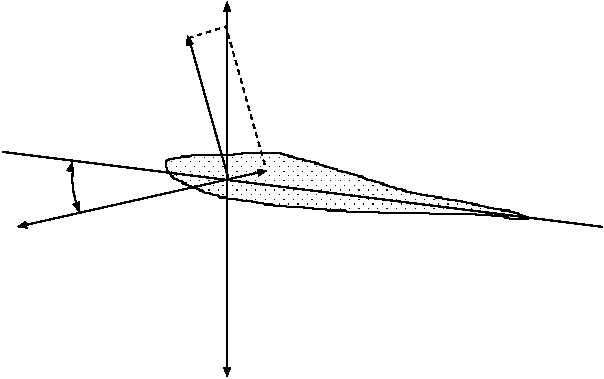
\includegraphics[clip]{youryoku}}%
  \caption{揚力の調整\label{fig:you}}%
 \end{center} 
\end{figure}

\end{document}